\section{Radio Interferometry}
\label{s:radio_astronomy}

\subsection{Radio Telescopes and its Resolution}
\label{s:radio_telescope}

\paragraph{}Angular resolution ($\theta$) of a telescope depends on the wavelength of light or 
radio waves ($\lambda$) and the diameter (D) of the telescope being used.
The relation between $\theta$, $\lambda$ and $D$ is given by
\begin{equation}
 \theta \sim  \lambda/D
\label{2.1}
\end{equation}
Here $\theta$ is in radians and $\lambda$ and $D$  in meters.

\paragraph{}Radio telescopes are used to study radio waves emitted by astronomical objects
of wavelengths roughly between about 10 meters and 1 millimeter. It is possible to 
observe radio waves from the ground as shown in the figure \ref{Fignasa}, spacecraft are needed to
observe astronomical objects in gamma rays, X-rays, UV, and IR, while ground observations 
are possible in the visible, some parts of the near IR, and the radio.
\begin{figure}[!htbp]
  \begin{center}
      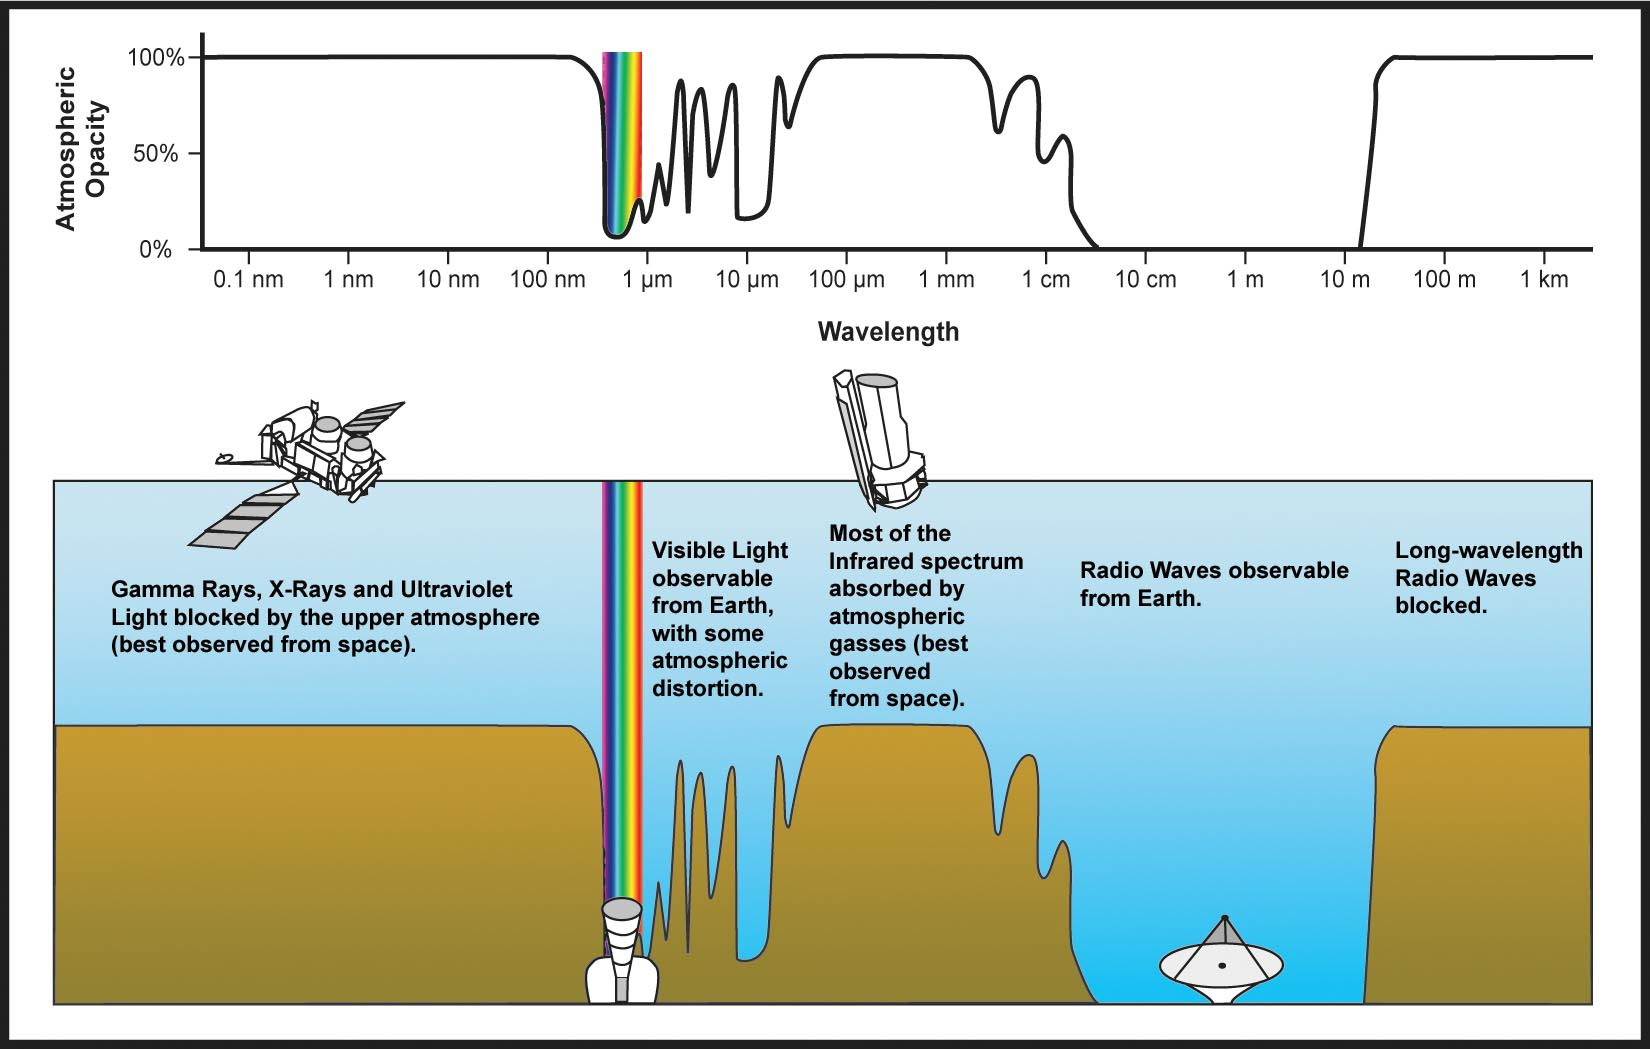
\includegraphics[width=6.1in,height=4in]{figures/nasa}
    \caption{Image credit : NASA/IPAC}
    \label{Fignasa}
  \end{center}
\end{figure}

\paragraph{}Due to larger operating wavelengths and primarily because of relation equation (\ref{2.1}), 
radio telescopes have to be much larger than optical telescopes to attain good angular resolution. Angular resolution 
is a measure of how small detail of an area in the sky can be seen. The larger the telescope, the more 
detail can be observed in a given wavelength.

\subsection{Radio Interferometry}
\label{s:radio_interferometry}

\paragraph{}Angular resolution of telescope given by equation (\ref{2.1}) is limited by its operating wavelength and 
diameter of aperture. To get good resolution, one has to either decrease the operating wavelength or 
increase the size of telescope. In radio astronomy, the wavelengths are so large that even though the 
sizes of radio telescopes are large, the angular resolution is poor as compared to optical instruments.
With these larger telescopes one can achieve higher resolutions by operating wavelengths in the
centimeter to millimeter range. Telescopes of hundreds of meters in diameter are needed to observe the source 
at metre wavelengths which would clearly impractical.

\paragraph{}Radio astronomers achieve higher resolution at metre wavelengths using a technique called 
\emph{Radio Interferometry}. The interferometers like GMRT (\cite{gmrt}) consist of array of antennas 
located on ground and resolution of such a telescope is proportional to maximum projected distance 
between the antennas. The separations between antennas are called as \emph{Baseline} and are measured in units of wavelength
($\lambda$). 

\subsubsection{Van Cittert \textendash Zernike theorem}

\paragraph{}Van Cittert \textendash Zernike theorem is the key theorem in radio interferometric imaging.
 It relates the spatial coherence function at two points on the ground also called Visibility function ($V(r_1,r_2)$)
 with the distribution of source intensity $I$. It also shows that the visibility function $V(r_1,r_2)$ depends only on the 
relative distances between two points i.e $r_1-r_2$

\paragraph{}As explained in \cite{ncrabookchap2}. Let us consider a two element interferometer with antenna 1 and antenna 2 
located on ground at $P_1(x_1,y_1,z_1)$ and $P_2(x_2,y_2,z_2)$ respectively. 
Consider an infinitesimal element of the source positioned at $P(x,y,z)$ in the sky shown in figure ().
If electric field intensity at the point $P$ is given by $\varepsilon(P)$, then the electric field at
the observation point $P_1$ \cite{wolf} is given by
\begin{equation}
 E(P_1) = \int \varepsilon(P) \frac{e^{-\frac{2\pi}{\lambda}D(P_1,P)}} {D(P_1,P)}d\Omega
\label{2.2}
\end{equation}
\paragraph{}where $D(P_1,P)$ is defined as the distance between the points $P$ and $P_1$. $\Omega$ is the solid 
angle subtend by the infinitesimal source at $P$.Assuming that the emission from the source is spatially incoherent,
at point $P_2$ the electric field is given by
\begin{equation}
 E(P_2) = \int \varepsilon(P) \frac{e^{-\frac{2\pi}{\lambda}D(P_2,P)}} {D(P_2,P)}d\Omega
\label{2.3}
\end{equation}

The spatial coherence function is given by
\begin{equation}
 < E(P_1)E^*(P_2)> = \int <\varepsilon(P)\varepsilon^*(P)> \frac{e^{-\frac{2\pi}{\lambda}(D(P_2,P)-D(P_2,P))}} {D(P_1,P) D(P_2,P)}d\Omega
\label{2.4}
\end{equation}

where Intensity($I$) of the source is defined as 
\begin{equation}
 I(P)=<\varepsilon(P)\varepsilon^*(P)>
\label{2.5}
\end{equation}

If we imagine a celestial sphere of radius $R$ and approximate the source lying on this sphere then we have $x=R cos(\theta_x)$
$y=R cos(\theta_y)$ and $z=R cos(\theta_z)$ where $cos(\theta_x),cos(\theta_y),cos(\theta_z)$ are direction cosine $l,m,n$.
Also $l^2+m^2+n^2=1$ and the solid angle $\Omega = \frac{dldm}{\sqrt{1-l^2-m^2}}$. Further \\\\
$
\begin{array}{rl}
  D(P_1,P) = &  [ (x-x_1)^2 + (y-y_1)^2 + (z-z_1)^2]^{\frac{1}{2}}\\
           = &  [ (Rl-x_1)^2 + (Rm-y_1)^2 + (Rn-z_1)^2 ]^{\frac{1}{2}}\\
	   = &  R[(l-x_1/R)^2 + (m-y_1/R)^2 + (n-z_1/R)^2 ]^{\frac{1}{2}}\\
	   \simeq & R [(l^2+m^2+n^2)-2/R(lx_1+my_1+nz_1)]^{\frac{1}{2}}\\
	   \simeq & R-(lx_1+my_1+nz_1)
\label{hello}
\end{array}
$\\
Similarly we have 
\begin{equation}
 D(P_2,P) = R-(lx_2+my_2+\sqrt{1-l^2-m^2}z_2)
\label{2.6}
\end{equation}
Using above equations we can approximate $D(P_1,P) D(P_2,P)$ as $R^2$ as shown below\\\\
$
\begin{array}{rl}
  D(P_1,P)D(P_2,P) =& \{R-(lx_1+my_1+nz_1)\}\{R-(lx_2+my_2+nz_2)\}\\
		   =& R(R-(l(x_1+x_2)+m(y_1+y_2)+z(z_1+z_2)) \\&+ (lx_2+my_2+nz_2)(lx_1+my_1+nz_1)
\end{array}
$\\\\
In above equation $R-(l(x_1+x_2)+m(y_1+y_2)+z(z_1+z_2) \simeq R$ and further \\$R^2>>(lx_2+my_2+nz_2)(lx_1+my_1+nz_1)$.
Hence we have 
\begin{equation}
 D(P_1,P)D(P_2,P) \simeq R^2
\label{2.7}
\end{equation}

Putting the above equations (\ref{2.5}),(\ref{2.7}) in equation (\ref{2.4}) we have
\begin{equation}
 < E(P_1)E^*(P_2)> = \frac{1}{R^2}\int I(P) e^{-\frac{2\pi}{\lambda}(l(x_2-x_1)+m(y_2-y_1)+n(z_2-z1))} \frac{dldm}{\sqrt{1-l^2-m^2}}
\label{2.8}
\end{equation}

Above equation () is the full Van Cittert-Zernike equation. It can be seen from above equation spatial coherence function or
visibility function $V(r_1,r_2)=< E(P_1)E^*(P_2)>$ depends upon $r_1-r_2$. We define baseline co-ordinates $u,v,w$ such that 
$u = (x_2-x_1)/\lambda$, $v = (y_2-y_1)/\lambda$ and $w = (z_2-z_1)/\lambda$ and also since we have relation $l^2+m^2+n^2=1$
the above equation reduced to
\begin{equation}
V(u,v,w) = \frac{1}{R^2}\int I(l,m) e^{-\frac{2\pi}{\lambda}(lu+mv+(\sqrt{1-l^2-m^2})w)} \frac{dldm}{\sqrt{1-l^2-m^2}} 
\label{2.9}
\end{equation}

\subsubsection{Two-Dimensional Approximation}

Equation (\ref{2.9}) under certain assumption can be approximated as two-dimensional Fourier transform of the source intensity
distribution. If we confined our observation to $u-v$ plane i.e when $w=0$ then we have 
\begin{equation}
V(u,v) = \frac{1}{R^2}\int I(l,m) e^{-\frac{2\pi}{\lambda}(ul+vm)} \frac{dldm}{\sqrt{1-l^2-m^2}} 
\label{2.10}
\end{equation}
Another approximation to above equation is when we consider that the source brightness distribution is limited only
to small region of sky. In this case $n =\sqrt{1-l^2-m^2} \simeq 1$. Then the equation (\ref{2.9}) becomes

\begin{equation}
V(u,v) = \frac{1}{R^2}\int I(l,m) e^{-\frac{2\pi}{\lambda}(ul+vm)} dldm
\label{2.11}
\end{equation}
Source brightness is described in $lm$ plane while the equivalent conjugate variables in Fourier space $u,v$ is
described in $uv$ plane.$u,v$ is interpreted as spatial frequency and Visibility function $V(u,v)$ as spatial
frequency spectrum of source brightness distribution. 


\subsection{Dirty Beam and Dirty Image}
\label{s:radio_dirty}

Fourier transform relation exists between source brightness $I$ and the visibility $V$ we can take 
an inverse Fourier transform which can be given by
\begin{equation}
 I(l,m) = \int_{-\infty}^{+\infty}\int_{-\infty}^{+\infty} V(u,v) e^{2\pi i (ul+vm)} dudv
\label{2.12}
\end{equation}
Since it is impractical to cover whole $uv$ plane, we measure visibilities only at some points. Due to which image of sky
is not the true image but comes with lot of noise such an image is called Dirty Image is given by 
\begin{equation}
 I^D(l,m) = \int_{-\infty}^{+\infty}\int_{-\infty}^{+\infty} S(u,v) V(u,v) e^{2\pi i (ul+vm)} dudv
\label{2.13}
\end{equation}
where $V(u,v)$ is observed visibility and $S(u,v)$ denote sampling function which is indicator of where
on $u-v$ plane visibilities are measured. It is given by 

\begin{equation}
S(u,v) = \delta(u-u_k,v-v_k)
\label{2.14}
\end{equation}

Hence practically we measure sampled Visibility function ($V^S(u,v)$) which is given by
\begin{equation}
V^S(u,v) = \delta(u-u_k,v-v_k)V(u_k,v_k)
\label{2.15} 
\end{equation}
 where $(u_k,v_k)$ are the co-ordinates of points where visibility is measured. Hence
the discretized form of visibility function with discretized $l-m$ grid with reference to equation (\ref{2.11}) is
given by
\begin{equation}
 V(u_j,v_j)= \displaystyle\sum\limits_{k=1}^{k=N} I(l_k,m_k) e^{2\pi i (u_jl_k+v_jm_k)}
 \label{extra}
\end{equation}
Note above equation denotes only one visibility at $(u_j,v_j)$.\\
In short we have $V^S = SV$. If $F$ denote Fourier operator then equation (\ref{2.13}) can be written as,
\begin{equation}
 I^D = FV^S = F(SV)
\label{2.16}
\end{equation}
By Convolution theorem (\cite{bracewell}),
\begin{equation}
 I^D = FS * FV
\label{2.17}
\end{equation}
For a point source of unit strength at $(l_0,m_0)$, $|V(u,v)=1|$\\
$FV= \delta(l-l_0,m-m_0)$\\
$I^D = FS * FV = FS * \delta =  FS$. \\This is called the Dirty Beam which is given by
\begin{equation}
 B =FS
\label{2.18}
\end{equation}
Hence putting equation (\ref{2.18}) in equation (\ref{2.17}). Dirty Image is defined as the 
convolution of dirty beam and true image ($FV$).
\begin{equation}
 I^D = B * FV
\label{2.19}
\end{equation}

\subsection{Deconvolution}
\label{s:radio_deconvolve}

\paragraph{}The deconvolution problem in equation (\ref{2.19}) corrects for the $u-v$
plane sampling effect. The lack of measurement at certain interferometric spacing means 
that in principle an infinite number of brightness distributions could be consistent with
our visibility data. On the other hand, we may incorporate additional information to constrain
our solutions. The most widely used deconvolution method are CLEAN (\cite{hogbom}) and Maximum
Entropy Minimization

\subsubsection{CLEAN Algorithm}
CLEAN algorithm consider sky as containing only isolated point sources and approximates an image by a collection of point sources.
It then deconvolve each point source using a simple iterative approach. The final deconvolved image which is also called CLEAN image 
is the sum of these CLEAN components convolved with a Gaussian beam. This algorithm was published by \cite{hogbom} in 1974 and several 
variations have been proposed since then. Following are the main steps of the CLEAN algorithm.
\begin{itemize}
 \item Find the peak in Dirty Image.
 \item Subtract a dirty beam ($B$) of approximate strength to remove its side-lobes.
 \item Construct CLEAN image $I'$ using position and magnitude of subtracted components.
 \item Continue looping until some threshold level is met.
 \item Convolve the final $I'$ with an idealized CLEAN beam.
\end{itemize}

\subsubsection{Maximum Entropy Minimization}

MEM method minimizes a smoothness function ("entropy") in an image.
Maximum entropy is also called the all-poles model or auto-regressive model.
For images with more than a million pixels, this algorithm is faster than CLEAN 
algorithm. Details of the algorithm can be found in \cite{}.

\subsection{GMRT}
\label{s:radio_gmrt}

\href{http://ncra.tifr.res.in}{National Centre for Radio Astrophysics ( NCRA )} has set up an international facility for radio astronomical research
in the metre wavelengths range of the radio spectrum known as the \href{http://gmrt.ncra.tifr.res.in}{Giant Metre wave Radio Telescope (GMRT)}. This is the
world's largest array of radio telescopes at metre wavelengths and is located at a site about 80 km north of Pune. 
GMRT consists of 30 fully steerable gigantic parabolic dishes of 45m diameter each spread over distances of upto 25 km.
There are fourteen telescopes randomly arranged in the central square 1 km by 1 km in size, with a further sixteen arranged
in three arms of a nearly "Y"-shaped array each having a length of 14 km from the array centre.

\begin{figure}[!htbp]
  \begin{center}
      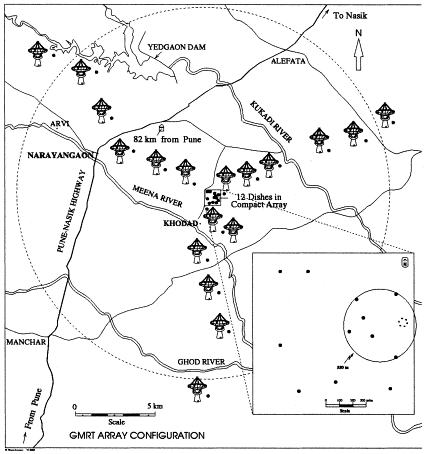
\includegraphics[height=6in]{figures/yshape}
    \caption{"Y" shaped Array}
    \label{FigYshape}
  \end{center}
\end{figure}

Antenna feeds at five different frequency centered at 153, 233, 327, 610, and 1420 MHz, with polarization. 
The maximum baseline in the array gives the telescope an angular resolution 
(the smallest angular scale that can be distinguished) of about 1 arc-second at the frequency of 1420 MHz.


\subsection{Compressed Sensing formulation for Radio Interferometry}
\label{s:radio_cs}
\paragraph{}Equation (\ref{2.11}) shows that under certain approximation, Visibility function is the Fourier transform of
source brightness. Radio Interferometers like GMRT measures visibility at very few points on $u-v$ plane.
At a time GMRT measures 435($C(30,2)$) visibilities. Each pair of antenna measures one visibility. This is 
shown in figure\footnote{Image by A.\ Basu, NCRA}(\ref{Figattime}) where each point represent one visibility.
\begin{figure}[!htbp]
 \hspace*{-10em}
 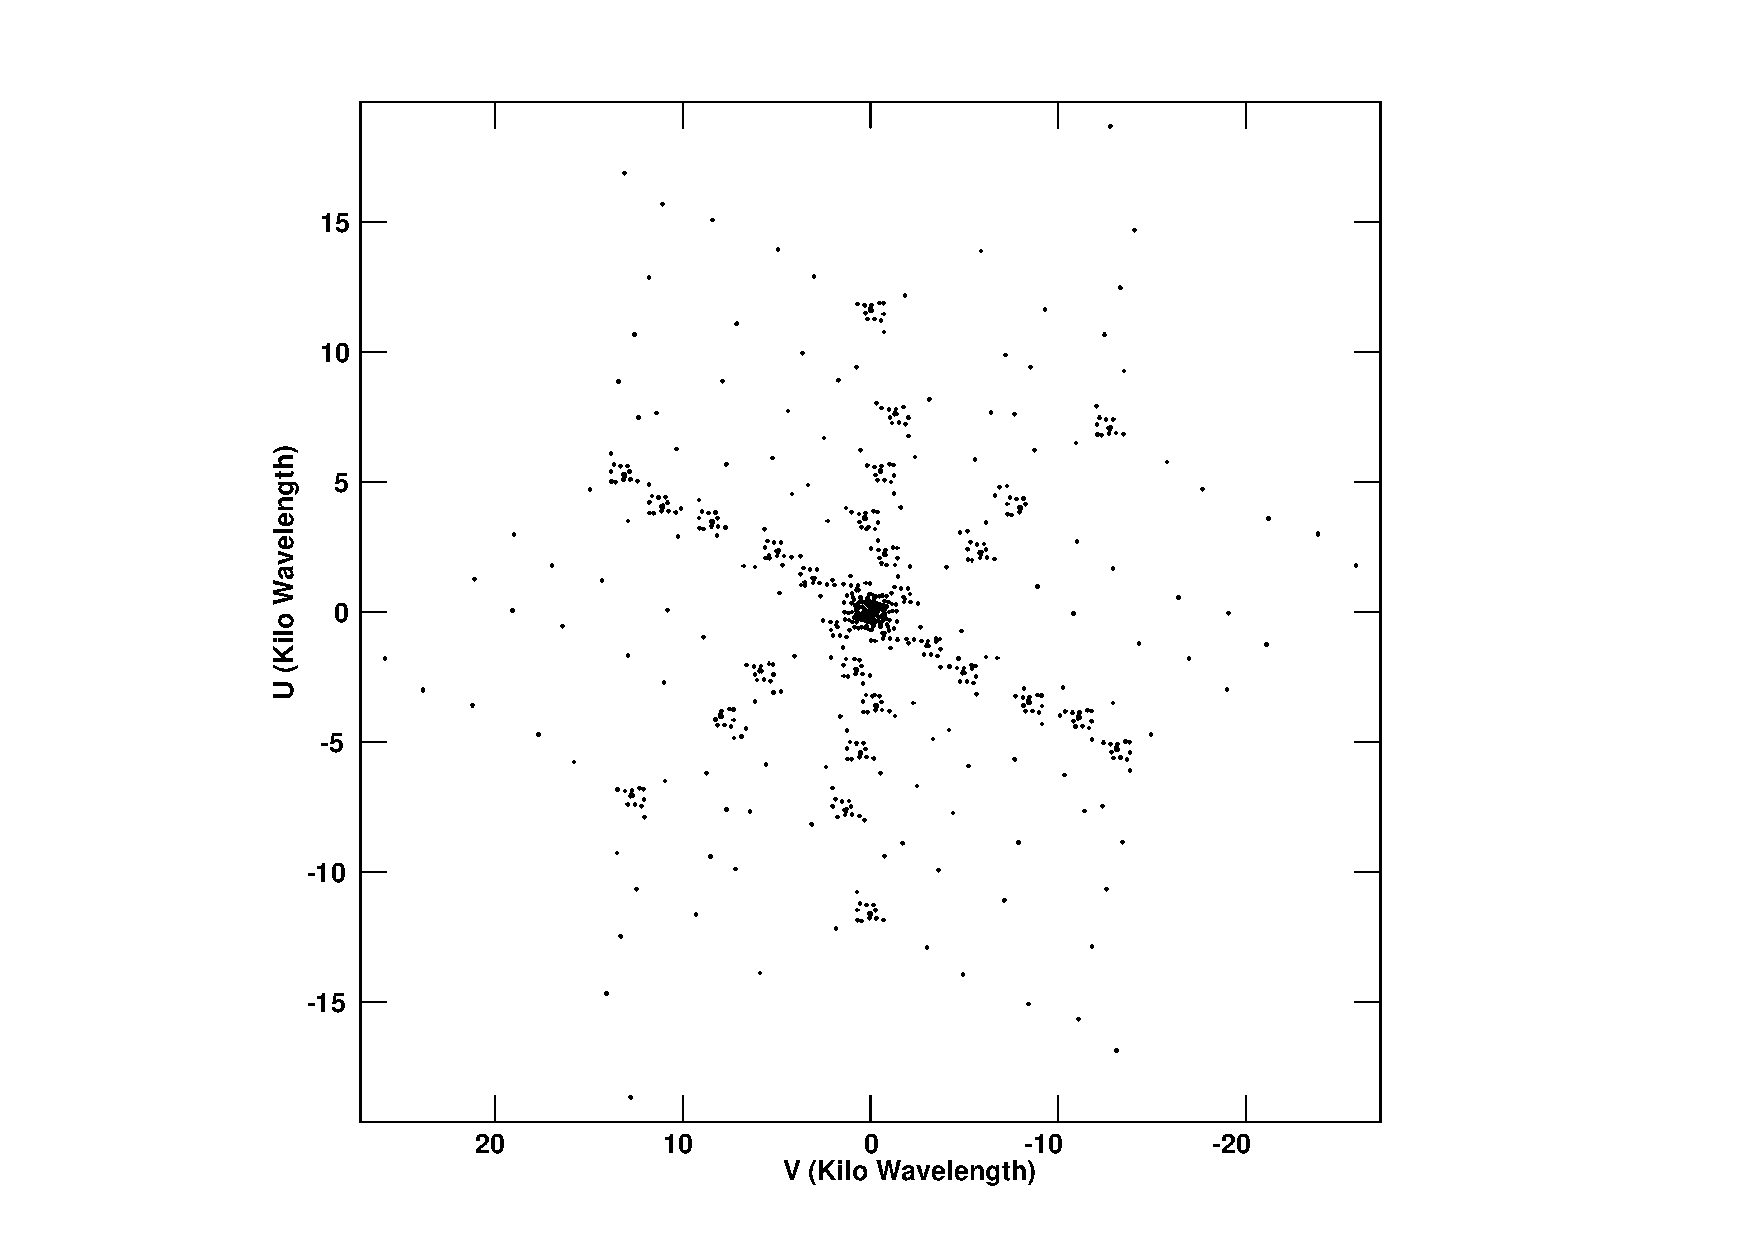
\includegraphics[width=1.5\textwidth]{figures/attime}
 \caption{$uv$ coverage at a time}
 \label{Figattime}
\end{figure}

% ------------------------------------------------------------------------
\begin{figure}[!htbp]
 \hspace*{-10em}
 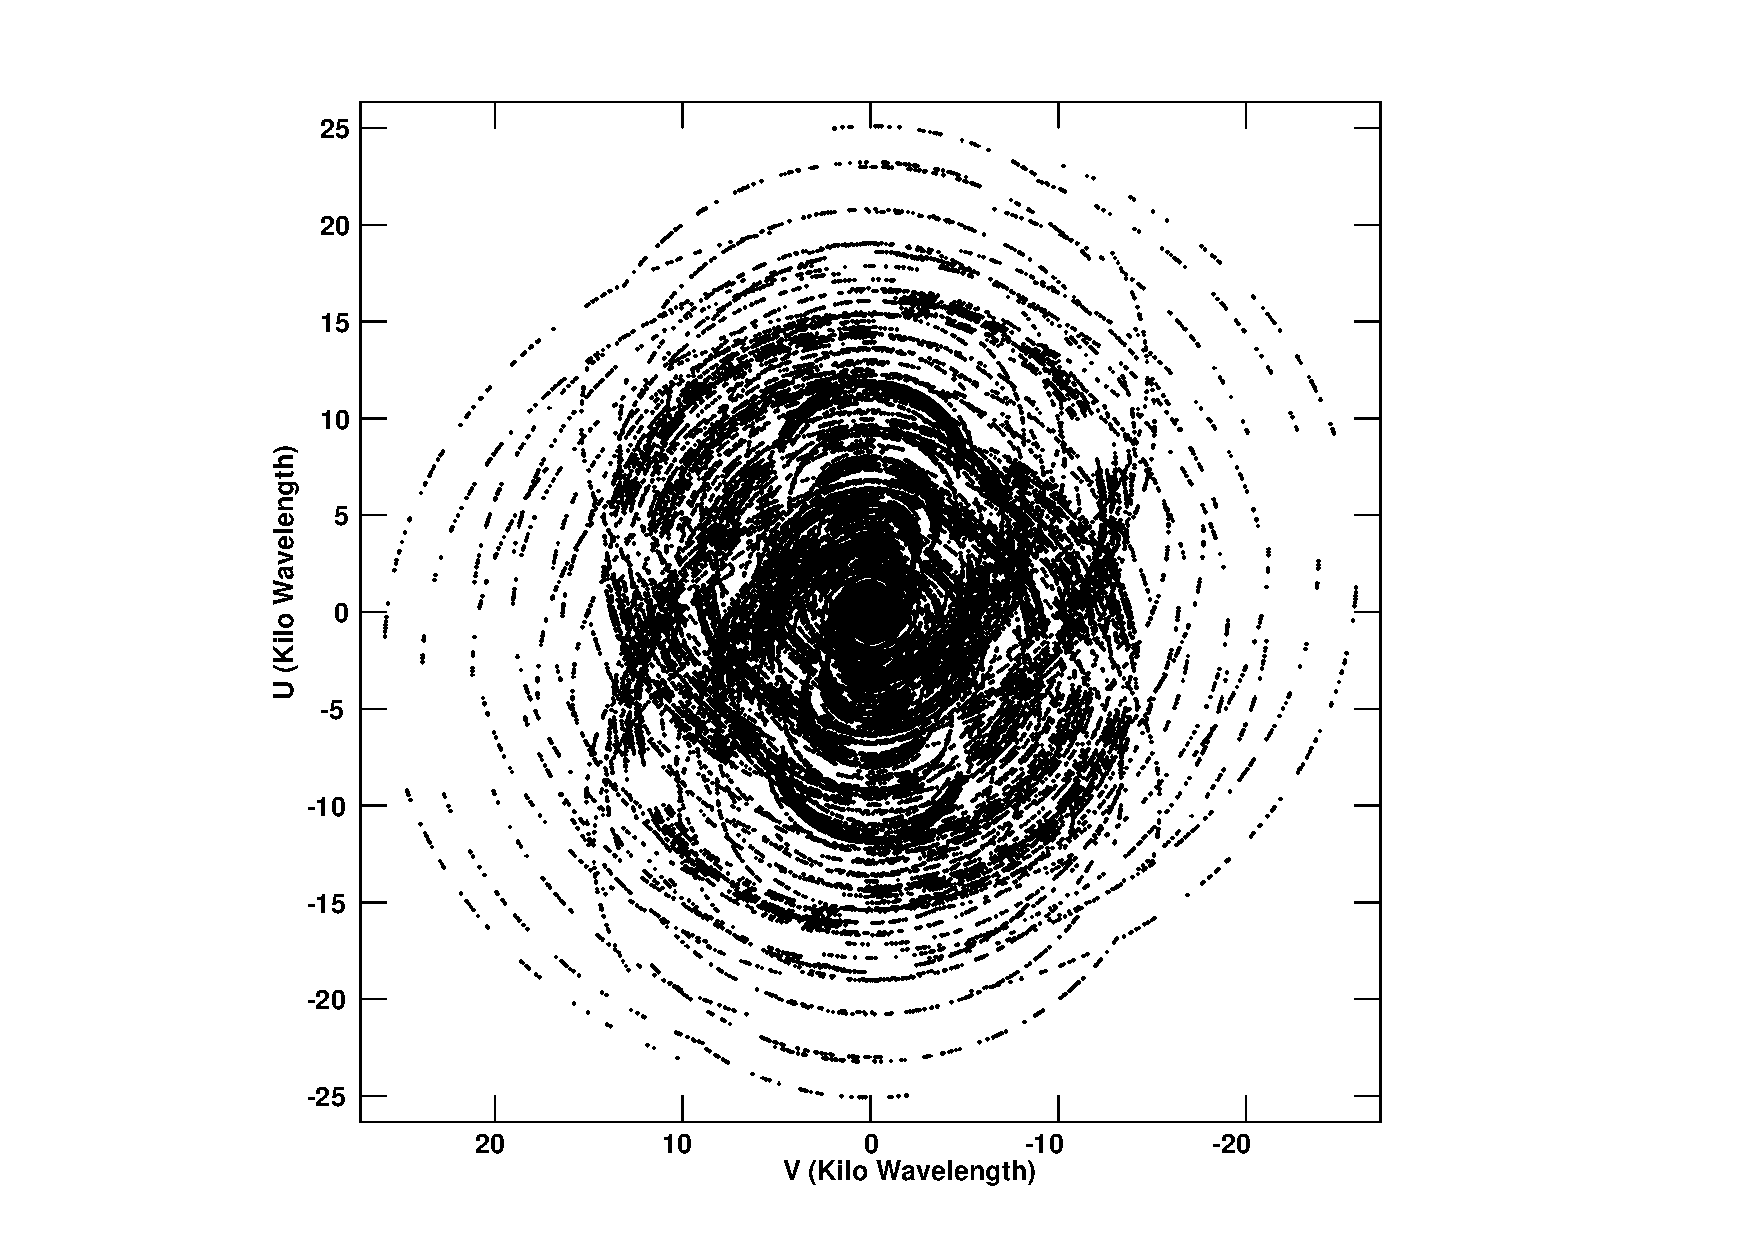
\includegraphics[width=1.5\textwidth]{figures/fewhrs}
 \caption{$uv$ coverage for few hours}
 \label{Figfewhrs}
\end{figure}
\newpage
\paragraph{}Due to rotation of earth, the projected separation between the antenna change and over certain time
it covers more point on the $u-v$ plane. This is shown in figure \footnote{Image by A.\ Basu, NCRA}(\ref{Figfewhrs})

\paragraph{}Even after few hours of $uv$ coverage (figure :\ref{Figfewhrs}) $uv$ coverage is not uniform.
Clearly we have under-sampled visibility data and hence Compressed Sensing methods proven to be viable option. Equation (\ref{2.11})
can be cast in to compressed sensing setting with visibilities as measurement vector and partial 2-D Fourier matrix as
measurement matrix and sky image as the unknown. In radio astronomy, most of the sources are point source so, most of the time
image is sparse in euclidean image. However there are the cases in which we have to represent image in some sparse basis which
can be done with some extra effort as in case of other application of compressed sensing.

\subsection{Why Compressed Sensing in Radio Astronomy?}
\label{s:radio_cs_why}
\paragraph{}In general, Compressed Sensing is advantageous when signals are sparse in some known basis, measurements are expensive and 
computations are cheaper at receiving end. These situations make Compressed Sensing methods a strong candidate for image 
deconvolution problem in radio astronomy. 
\paragraph{}Compressed Sensing methods can directly reconstruct the image from the sparse observations, without the need 
for an iterative deconvolution. Also it will be very efficient technique, when the 2-D approximation to Van Cittert-Zernike Theorem
breaks. Further with the advent of recent efficient and robust $\ell_1$ based algorithms, Compressed Sensing
takeover mainstream deconvolution methods used in Radio Astronomy like CLEAN and Maximum Entropy minimization as discussed 
in section 2.4. 










% ------------------------------------------------------------------------

%%% Local Variables: 
%%% mode: latex
%%% TeX-master: "../thesis"
%%% End: 
